\section{Thực nghiệm và đối sánh}
\label{sec:experiments}

\subsection{Thiết lập}

Mọi phép đo chạy trên Apple M1 (16 GB RAM), macOS, Python 3.14.7. Bộ đo \texttt{bench/run.py} chạy mỗi cấu hình
(thí nghiệm, biến thể, kích thước) trong \emph{một subprocess riêng}, để bộ nhớ và bộ đệm của lần đo trước
không ảnh hưởng lần sau. Phần dựng dữ liệu không tính giờ. Thời gian là trung vị của 5 lần chạy, đo bằng
\texttt{time.perf\_counter}. Bộ nhớ là đỉnh cấp phát của riêng giải thuật, đo bằng \texttt{tracemalloc} trong một lần chạy
thứ sáu. Mỗi cấu hình có giới hạn 120~giây, quá giới hạn thì ghi \emph{timeout} và vẫn giữ trong bảng. Mọi bộ dữ liệu
sinh với seed cố định nên chạy lại cho cùng kết quả.

\textbf{Bộ dữ liệu.}
(1) \emph{Bản đồ thật}: 38\,604 Intersection, 69\,411 Road Segment (Mục~\ref{sec:graph}).
(2) \emph{Đồ thị dạng mạng đường}: lưới $k\times k$ lệch ngẫu nhiên, mỗi đỉnh có cạnh hai chiều tới 4 láng giềng và thêm
cạnh một chiều tới các đỉnh lân cận cho đủ 5 cạnh ra. Như vậy $E\approx 5V$, với $V$ từ 961 đến 49\,729 (10\,000 đỉnh ứng
với 50\,000 cạnh, đúng quy mô đề yêu cầu).
(3) \emph{Đồ thị dày}: mỗi đỉnh có $V/4$ cạnh ra với trọng số ngẫu nhiên, $V\le 2000$, tức $E$ tới gần $10^6$.
(4) \emph{Đồ thị Hub đầy đủ}: 50 đến 400 điểm ngẫu nhiên trong mặt phẳng.
(5) \emph{Bài toán xếp hàng}: khối lượng 1--100~kg (đơn vị 0{,}1~kg), cước 10--500 nghìn đồng,
$W=\min(15\,000,\ \sum w_i/2)$.
(6) \emph{Ma trận TSP bất đối xứng}: khoảng cách Euclid, mỗi chiều nhân một hệ số ngẫu nhiên riêng trong $[1;1{,}6]$.

\textbf{Baseline.} Đề yêu cầu so sánh với cấu trúc cơ bản (mảng, danh sách). Vì vậy mỗi thí nghiệm có một biến thể
dựa trên mảng: Dijkstra chọn đỉnh bằng mảng $O(V^2)$, Quick-Find, Prim mảng, vét cạn. Hàng đợi \texttt{heapq} của Python
viết bằng C nên chỉ được vẽ làm \emph{đường tham chiếu} (nét chấm). So sánh nó với heap viết bằng Python thuần là so sánh
trình thông dịch với mã máy, không phải so sánh giải thuật.

\subsection{Đường đi ngắn nhất}

\begin{table}[t]
\centering
\caption{SSSP trên bản đồ thật (38\,604 đỉnh, 69\,411 cạnh), một nguồn, toàn bộ đồ thị}
\label{tab:sssp-osm}
\begin{tabular}{lrrr}
\toprule
Biến thể & Thời gian & Bộ nhớ & Heap lớn nhất \\
\midrule
Dijkstra + Adaptable Heap & 115{,}3 ms & 3\,956 KB & 276 \\
Dijkstra + Standard Heap (lazy) & 94{,}5 ms & 1\,544 KB & 289 \\
\texttt{heapq} (C, tham chiếu) & 35{,}7 ms & 1\,204 KB & -- \\
Dijkstra + mảng $O(V^2)$ & timeout & -- & -- \\
Bellman-Ford (dừng sớm) & 2\,957 ms & 2\,705 KB & -- \\
\bottomrule
\end{tabular}
\end{table}

\begin{figure}[t]
\centering
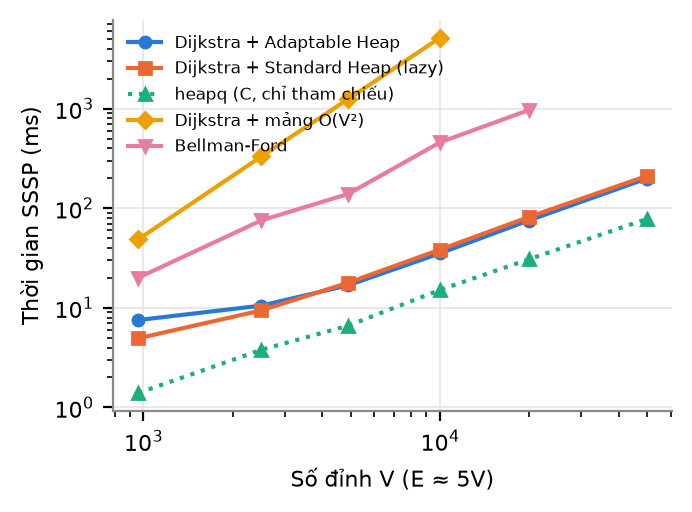
\includegraphics[width=\columnwidth]{sssp_time}
\caption{Thời gian SSSP trên đồ thị dạng mạng đường ($E\approx 5V$, thang log--log).}
\label{fig:sssp-time}
\end{figure}

\begin{figure*}[t]
\centering
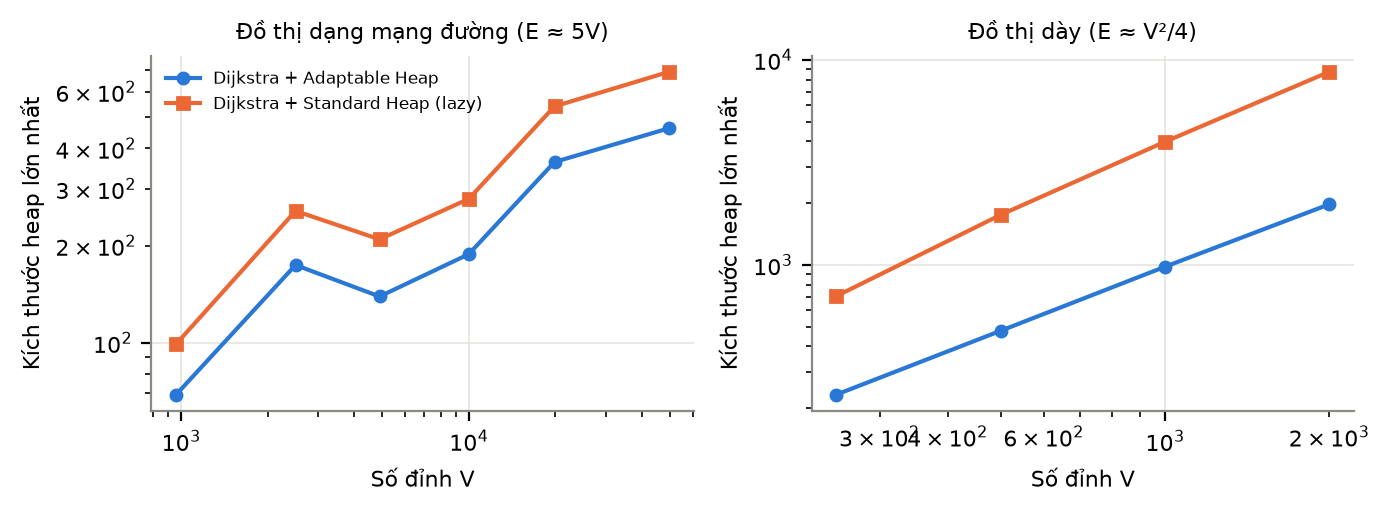
\includegraphics[width=0.49\textwidth]{heap_peak}\hfill
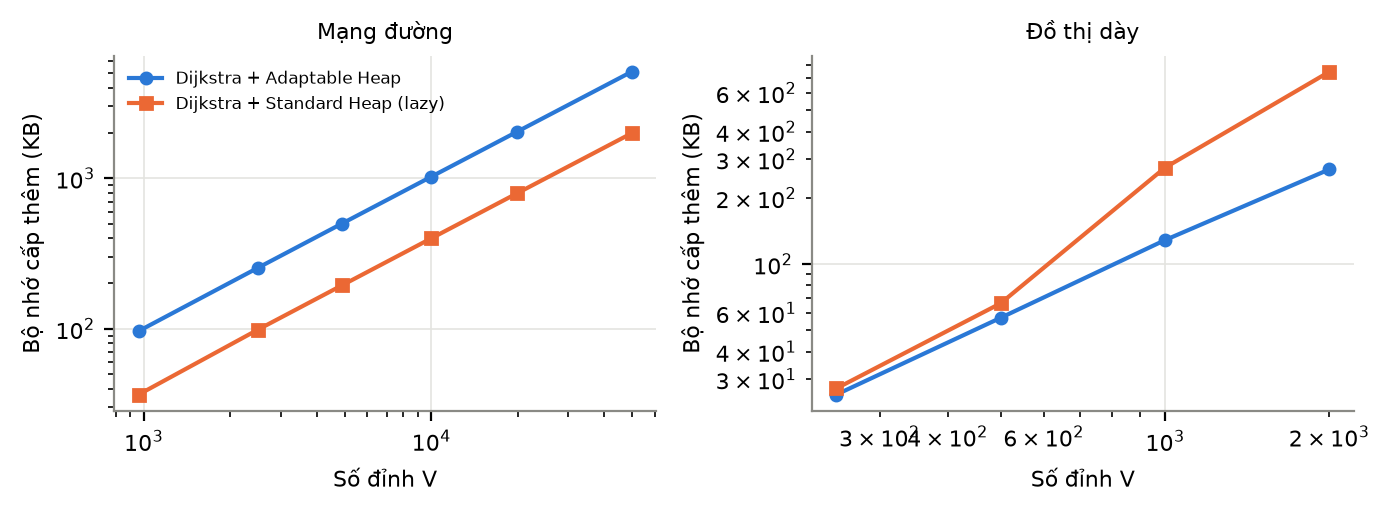
\includegraphics[width=0.49\textwidth]{sssp_memory}
\caption{Trái: kích thước heap lớn nhất. Phải: bộ nhớ cấp thêm. Ở mỗi hình, panel trái là đồ thị dạng mạng đường,
panel phải là đồ thị dày.}
\label{fig:heap}
\end{figure*}

Bảng~\ref{tab:sssp-osm} và Hình~\ref{fig:sssp-time} cho ba nhận xét.

\textbf{(i) Trên mạng đường, lazy heap không phình to.} Về lý thuyết, lazy heap có thể chứa tới $E$ phần tử. Thực tế, ở
$V=49\,729$ heap lớn nhất chỉ có 691 phần tử, còn heap của Adaptable Heap có 462 phần tử, tức dưới 1{,}5\% số đỉnh
(Hình~\ref{fig:heap}). Lý do: đồ thị đường bộ gần phẳng và bậc nhỏ, nên tập đỉnh đang chờ của Dijkstra chỉ là một "mặt sóng"
mỏng quanh nguồn. Khi số phần tử trùng lặp ít, lợi thế cận $O(V)$ của Adaptable Heap không thể hiện ra. Ngược lại, mỗi đỉnh
được chạm tới đều cần một đối tượng Locator, nên Adaptable Heap tốn bộ nhớ gấp khoảng 2{,}5 lần (5\,099 KB so với 1\,989 KB)
và chậm hơn 5--20\%. Hai đường thời gian gần như trùng nhau và cùng tăng tuyến tính theo $V$ trên thang log, khớp với cận
$O((V+E)\log V)$.

\textbf{(ii) Trên đồ thị dày, Adaptable Heap thắng.} Mỗi đỉnh có $V/4$ cạnh vào, nên decrease-key xảy ra liên tục. Ở
$V=2000$ ($E\approx 10^6$), lazy heap đạt 8\,737 phần tử so với 1\,974 của Adaptable Heap (gấp 4{,}4 lần) và dùng
747 KB so với 269 KB. Adaptable Heap nhanh hơn 16\% (123{,}6 ms so với 146{,}6 ms). Như vậy lợi ích của Locator phụ thuộc vào
\emph{tỉ lệ decrease-key trên số đỉnh}, không phải lúc nào cũng có.

\textbf{(iii) Baseline.} Dijkstra dùng mảng $O(V^2)$ chậm hơn 146 lần ở $V=10\,000$ (5{,}14 s so với 35 ms) và quá
120~s trên bản đồ thật. Kể cả trên đồ thị dày, nơi $O(V^2)$ về lý thuyết là tối ưu, bản mảng vẫn chậm gấp 2{,}8 lần, vì vòng
quét $V$ phần tử chạy hoàn toàn trong trình thông dịch. Bellman-Ford dừng sớm chậm hơn 13 lần ở $V=10\,000$ và 26 lần trên
bản đồ thật. Nó không bị chậm tới mức $O(VE)$ đầy đủ vì số vòng lặp chỉ bằng số cạnh của đường đi ngắn nhất dài nhất.
\texttt{heapq} nhanh hơn heap Python của nhóm 2{,}6--3{,}2 lần ở mọi kích thước. Đây là hằng số của mã C, còn độ dốc của hai
đường như nhau.

\textbf{Reroute.} Trên bản đồ thật, một Traffic Incident nằm ngoài tuyến được bỏ qua sau 0{,}4 ms (chỉ kiểm tra mặt nạ
\texttt{on\_route}). Một sự cố trên tuyến buộc phải chạy lại Dijkstra từ vị trí xe, mất khoảng 100--110 ms. Đây là số đo từ
một lần thao tác trên giao diện demo, chưa phải trung vị nhiều lần, nhưng chênh lệch hơn hai bậc là đúng như phân tích
$O(L)$ so với $O((V+E)\log V)$.

\begin{figure}[t]
\centering
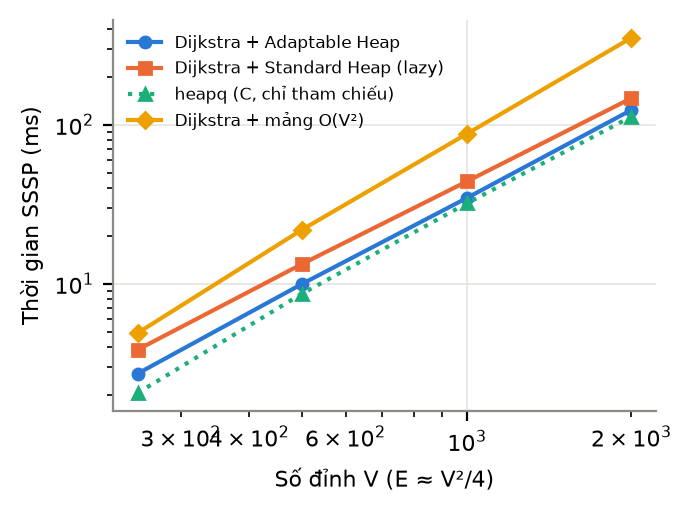
\includegraphics[width=\columnwidth]{sssp_dense_time}
\caption{SSSP trên đồ thị dày ($E\approx V^2/4$).}
\label{fig:dense}
\end{figure}

\subsection{Union-Find}

\begin{figure*}[t]
\centering
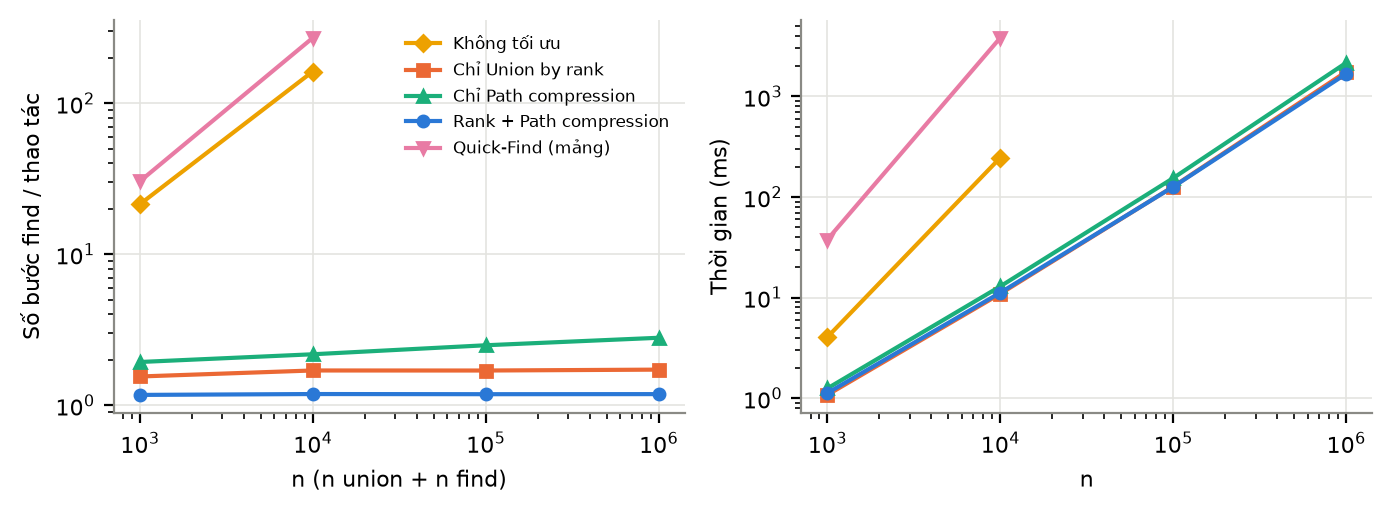
\includegraphics[width=0.49\textwidth]{dsu}\hfill
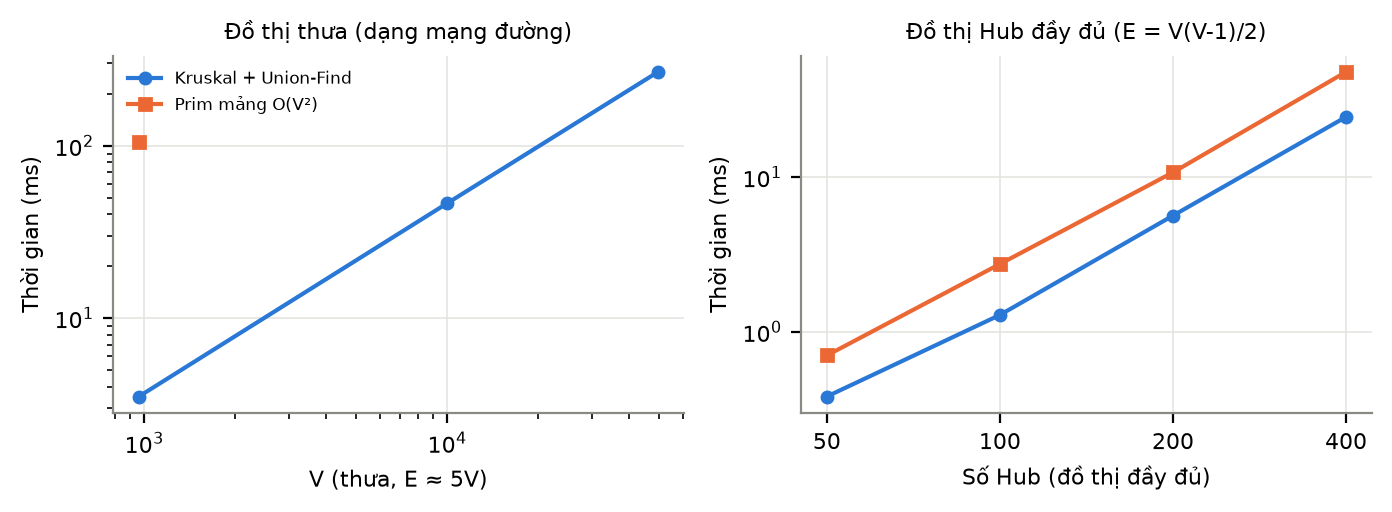
\includegraphics[width=0.49\textwidth]{mst}
\caption{Trái: Union-Find với $n$ phép union và $n$ phép find ngẫu nhiên (số bước trên một thao tác; thời gian).
Phải: thời gian tìm MST trên đồ thị thưa và đồ thị Hub đầy đủ.}
\label{fig:dsu-mst}
\end{figure*}

\begin{table}[t]
\centering
\caption{Số bước duyệt con trỏ \texttt{parent} trung bình trên một thao tác}
\label{tab:dsu}
\begin{tabular}{lrrrr}
\toprule
Biến thể & $n=10^3$ & $10^4$ & $10^5$ & $10^6$ \\
\midrule
Rank + Path compression & 1{,}17 & 1{,}19 & 1{,}18 & 1{,}19 \\
Chỉ Union by rank & 1{,}55 & 1{,}70 & 1{,}70 & 1{,}72 \\
Chỉ Path compression & 1{,}93 & 2{,}18 & 2{,}50 & 2{,}80 \\
Không tối ưu & 21{,}4 & 162 & timeout & -- \\
Quick-Find (số lần ghi) & 30{,}4 & 271 & -- & -- \\
\bottomrule
\end{tabular}
\end{table}

Bảng~\ref{tab:dsu} là minh chứng thực nghiệm cho cận khấu hao $O(\alpha(n))$. Khi bật cả hai tối ưu, số bước trên một thao
tác giữ ở 1{,}17--1{,}19 trong khi $n$ tăng 1000 lần. Thời gian tăng tuyến tính theo số thao tác: 1{,}68 s cho $2\cdot 10^6$
thao tác, tức khoảng 0{,}84~$\mu$s mỗi thao tác. Chỉ dùng path compression thì số bước tăng chậm, đúng với cận
$O(\log n)$ khấu hao. Chỉ dùng union by rank thì số bước ổn định ở mức cao hơn, vì chiều cao cây bị chặn bởi $\log_2 n$ nhưng
không giảm đi. Bản không tối ưu tăng gần tuyến tính và quá thời gian ở $n=10^5$. Quick-Find tốn 3{,}8 s ở $n=10^4$, chậm hơn
bản tối ưu 340 lần, vì mỗi phép union phải gán lại nhãn cho tới $n$ phần tử.

\subsection{Cây khung nhỏ nhất}

Kruskal và Prim luôn cho cùng tổng trọng số, đây cũng là cách kiểm tra chéo tính đúng. Trên đồ thị thưa, Kruskal xử lý
49\,729 đỉnh và 248\,645 cạnh trong 268 ms. Prim mảng cần ma trận $V\times V$, mất 105 ms ngay ở $V=961$ và quá thời gian
ở $V=10\,000$. Trên đồ thị Hub đầy đủ, ta dự đoán Prim $O(V^2)$ sẽ thắng Kruskal $O(V^2\log V)$, nhưng số đo cho thấy
\emph{Kruskal vẫn nhanh hơn khoảng 2 lần} (24{,}5 ms so với 48{,}0 ms ở 400 Hub). Nguyên nhân: bước sắp xếp
$O(E\log E)$ của Kruskal dùng \texttt{list.sort} viết bằng C, còn vòng $O(V^2)$ của Prim là Python thuần. Ở quy mô vài trăm
Hub, hệ số $\log V\approx 9$ nhỏ hơn chênh lệch hằng số giữa C và Python. Đây là một ví dụ cho thấy cận tiệm cận chỉ dự đoán
xu hướng khi $n$ đủ lớn, không dự đoán thứ hạng ở một kích thước cụ thể. Trong demo, Backbone giữa 24 Hub mất 3{,}8 s, gần
như toàn bộ là 24 lần Dijkstra để dựng ma trận; riêng phần MST không đáng kể.

\subsection{Xếp hàng lên xe và thứ tự giao}

\begin{figure}[t]
\centering
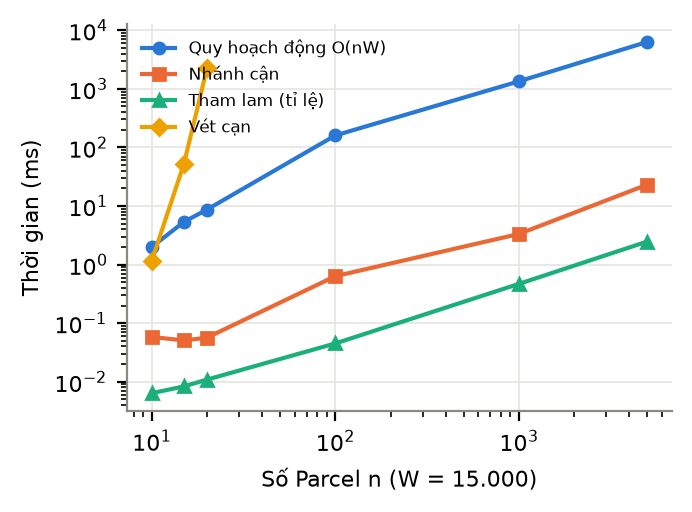
\includegraphics[width=\columnwidth]{knapsack}
\caption{Thời gian giải 0/1 Knapsack, $W=15\,000$ (xe 1{,}5 tấn).}
\label{fig:knapsack}
\end{figure}

\textbf{Knapsack} (Hình~\ref{fig:knapsack}). Khi $W$ cố định, thời gian quy hoạch động tăng tuyến tính theo $n$: 160 ms,
1{,}34 s và 6{,}33 s với $n=100$, 1000 và 5000. Bảng truy vết chiếm 2 MB, 15 MB và 74 MB, khớp với $n(W+1)$ byte. Vét cạn
tăng gấp đôi khi thêm mỗi Parcel và mất 2{,}2 s ở $n=20$. Nhánh cận chỉ mất 3{,}3 ms ở $n=1000$ và 23 ms ở $n=5000$, nhanh
hơn quy hoạch động tới 270 lần. Kết quả này chỉ đúng cho dữ liệu ngẫu nhiên, khi khối lượng và cước độc lập nhau, nên cận
phân số cắt nhánh rất sớm. Trường hợp xấu nhất của nhánh cận vẫn là hàm mũ, và nhóm chưa thử bộ dữ liệu có khối lượng và cước
tương quan chặt (trường hợp khó cho nhánh cận). Tham lam theo tỉ lệ thiếu 5{,}9\% so với tối ưu ở $n=10$, nhưng chỉ còn
0{,}05\% ở $n=5000$: khi có nhiều Parcel nhỏ so với $W$, phần dư cuối cùng không đáng kể.

\begin{figure}[t]
\centering
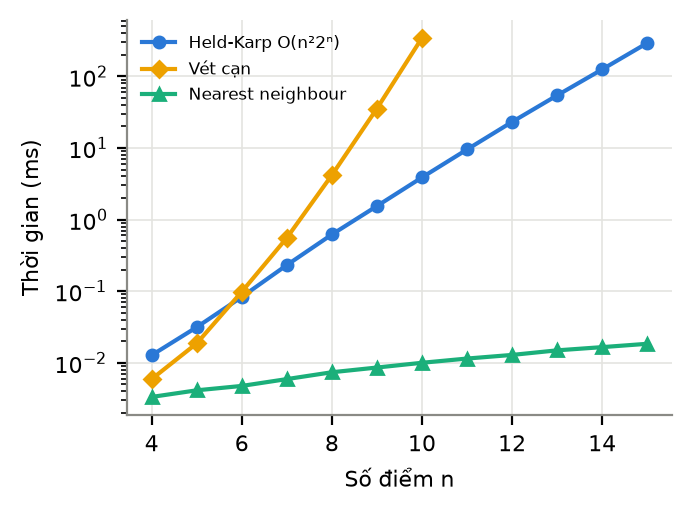
\includegraphics[width=\columnwidth]{tsp}
\caption{Thời gian TSP bất đối xứng (thang log): Held-Karp, vét cạn, nearest neighbour.}
\label{fig:tsp}
\end{figure}

\textbf{TSP} (Hình~\ref{fig:tsp}). Held-Karp tăng khoảng 2{,}3 lần mỗi khi thêm một điểm và mất 293 ms ở $n=15$. Vét cạn tăng
khoảng $n$ lần mỗi bước và đã mất 345 ms ở $n=10$. Ở cùng $n=10$, Held-Karp nhanh hơn 89 lần (3{,}9 ms). Nearest neighbour gần
như tức thời nhưng dài hơn tối ưu 5--41\% (trung bình 21\%). Với một chuyến giao, chênh lệch đó tương đương vài chục phút chạy
xe. Vì vậy giới hạn 12 điểm mỗi chuyến (khoảng 23 ms) là điểm cân bằng hợp lý giữa tối ưu và thời gian phản hồi.

\subsection{Giới hạn của thực nghiệm}

(1) Mọi cài đặt viết bằng Python, nên hằng số của trình thông dịch có thể làm đảo thứ hạng so với lý thuyết, như đã thấy ở
Prim và Kruskal. (2) Chỉ đo trên một máy. (3) \texttt{tracemalloc} chỉ đếm bộ nhớ do Python cấp phát, không đếm bộ nhớ của
tiến trình. (4) Đỉnh của bản đồ thật gồm cả điểm uốn của đường, nên số đỉnh lớn hơn số giao lộ thật. (5) Vận tốc là giả định
theo loại đường, chưa có dữ liệu giao thông thực tế. (6) Thời gian reroute là số đo trên demo, chưa lặp lại nhiều lần.
